\chapter{绪论}

\section{研究背景与意义}

信息化战争形态的持续演进和多域作战理念的深入发展,使得战术数据链(Tactical Data Link, TDL)已成为现代联合作战体系中实现信息共享、态势感知与指挥控制的核心基础设施\cite{NDIA_PMW101_2024,NDIA_PMW101_2022}。作为其中的典型代表,{Link16} 基于 MIL-STD-6016 消息标准,以 J 系列报文为核心,实现了跨平台、跨军种、跨域的信息交互与协同作战\cite{DOTE_2022_MIDS_LVT,NAVAIR_MIDS_Overview}。

然而,作战环境的复杂化和通信需求的多样化,使得现有战术数据链系统正面临新的技术挑战。{Link16} 系统在复杂电磁环境下的信号检测与识别能力仍存在瓶颈,难以满足高动态、多干扰环境下的通信稳定性需求\cite{AviationWeek_SDA_LEO_2024,SDA_testing_OK_2023}。同时,天基拓展和超视距通信需求对传统链路结构提出了更高要求,促使数据链系统向分布式与智能化方向演进\cite{MIL_STD_6016_Active_2024,L3Harris_MIDS_JTRS_2021}。此外,多链路并行应用和跨域作战的普及,使得不同标准协议之间的融合与互操作成为制约系统协同效能提升的关键问题。

基于上述背景,构建基于 MIL-STD-6016 的战术数据链信息标准数据库并引入微服务化与自动化设计理念,具有重要的理论价值与工程意义。

(1)理论价值:通过系统梳理和数据库化建模 MIL-STD-6016 消息体系,可实现消息、字段、编码规则的统一存储与规范化管理,为战术数据链标准体系研究提供结构化的数据支撑。通过建立语义概念绑定与跨标准映射机制,能够实现 MIL-STD-6016、MQTT、MAVLink 等协议间的语义对齐与信息互通,为跨链互操作与语义融合理论提供新的研究思路。基于数据库语义层的统一模型可为后续标准化仿真与知识图谱构建提供理论基础。

(2)工程意义:基于云原生与微服务架构的数据库系统,可实现服务模块的独立部署、弹性扩展与容错恢复,显著提升系统可维护性与可靠性。通过引入容器化与 CI/CD 自动化部署机制,系统可实现持续集成与快速迭代,满足复杂通信体系下的动态部署需求。数据库与仿真系统的深度集成能够支撑态势信息处理、多链融合验证及装备互操作性测试,为构建智能化、可扩展的战术通信体系提供坚实的工程支撑。

\section{国内外研究现状}

\subsection{战术数据链}

战术数据链技术起源于上世纪七十年代的联合战术信息传输需求。美国及北约成员国先后发布了多项核心标准,如 MIL-STD-6016、MIL-STD-3011(JREAP)和 STANAG 5516\cite{丁丁2019,马建强2020},形成了以 J 系列报文为核心的数据交换体系。这些标准不仅规范了消息格式、通信协议和互操作流程,也确立了数据链在联合作战中的通用语言地位。MITRE、NATO C3 Agency 等研究机构在此基础上提出了多链路融合与跨标准数据映射的研究框架\cite{程方昊2025,陈利玲2025},通过构建标准化信息模型实现了 Link11、Link16、Link22 等链路之间的数据互通。L3Harris 的 MIDS 终端与 Collins Aerospace 的 TTR 系统已实现链路消息解析、协议转发和仿真验证,为多平台装备间的实时协同奠定了技术基础。这些成果标志着国外战术数据链体系已从链路互通向语义级协同演进,研究重心逐步转向体系融合与信息标准化。

图\ref{fig_tactical_datalink_research_status}展示了战术数据链研究现状的发展脉络,清晰呈现了国内外研究的发展历程和技术演进趋势。该图从时间维度展示了国外研究从1970年代的标准建立到2010年代至今的语义协同演进,以及国内研究从1990年代的防务电子化建设到2020年代至今的体系化发展,体现了技术发展的连续性和阶段性特征。

\begin{figure}[H]
    \centering
    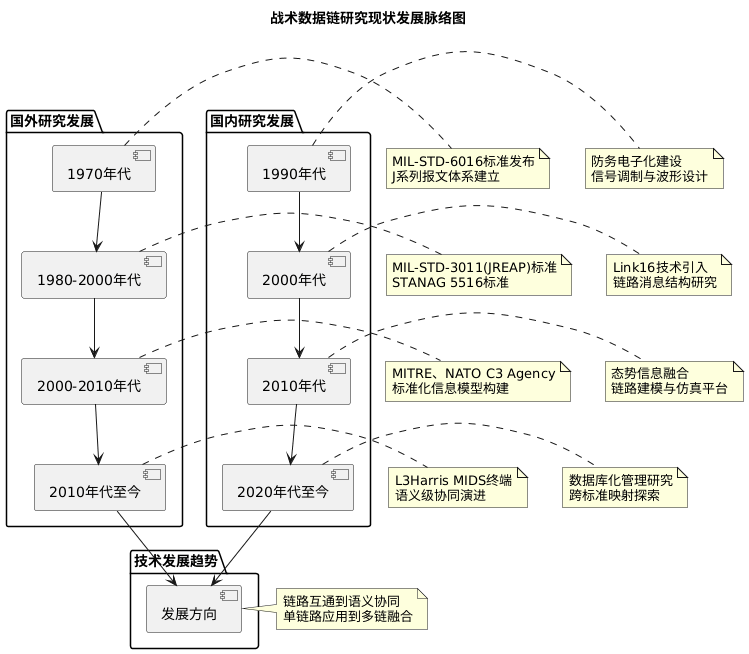
\includegraphics[width=0.9\textwidth,height=0.6\textheight,keepaspectratio]{chapters/fig-0/tactical_datalink_research_status.png}
    \caption{战术数据链研究现状发展脉络图}
    \label{fig_tactical_datalink_research_status}
\end{figure}

我国对战术数据链的研究始于上世纪九十年代的防务电子化建设阶段。最初的研究主要集中在信号调制、波形设计及抗干扰建模等底层通信环节\cite{wray_sheppard_1986_jtids_nav,ranger1996_jn}。21 世纪后,伴随 {Link16} 技术的引入,国内学界与科研机构开始系统研究链路消息结构、报文解析与仿真验证技术\cite{fried1978_taes,fried1984_navigation}。近十年来,研究范围逐步拓展至态势信息融合、链路建模与仿真平台建设等方向\cite{doherty1988_jn,L3Harris_MIDS_LVT_2025}。多个研究团队先后开发了用于消息格式验证、链路转发测试及通信性能评估的原型系统,初步具备了数据链标准化和协议适配的工程能力。然而,目前国内研究仍以特定标准或单链路应用为主,数据库化管理与跨标准映射研究尚未形成统一体系,缺乏对 MIL-STD-6016 消息的系统化建模与语义抽象机制,导致不同链路间数据融合与互操作效率仍受限制。

总体来看,国外在战术数据链领域已形成"标准主导—模型驱动—体系集成"的研究格局,而我国研究正在由"信号验证—系统开发—标准化建模"逐步转向体系化、架构化方向。未来的发展趋势是实现从链路互通到语义协同的跃迁,通过标准数据库建设与体系互操作机制,为多域作战提供统一的信息支撑平台。

\subsection{微服务架构}

微服务架构(Microservice Architecture, MSA)作为软件工程领域的重要演进方向,其理论基础可追溯至 2010 年前后。James Lewis 与 Martin Fowler 于 2014 年系统阐述了微服务概念,他们认为微服务是一种以业务能力为核心的分布式架构模式,强调服务自治、松耦合与独立部署。与传统单体应用相比,微服务能够在快速迭代与持续交付中保持模块独立性,从而显著提升系统的灵活性与可维护性。2015 年被称为"微服务元年",Netflix、Amazon、Google 等企业率先在大规模分布式系统中采用微服务架构,通过构建服务注册中心、API 网关与容错机制,实现了服务治理、动态伸缩与高可用部署,推动了这一理念从企业实践走向学术研究的深入阶段。

2018–2020 年期间,国外学术界开始聚焦于微服务的系统化研究与性能分析。Waseem 等人基于 106 份工业问卷与多项访谈,系统总结了微服务系统的设计、监控与测试现状。他们指出,领域驱动设计(DDD)与基于业务能力的服务划分已成为主流方法,API 网关与 Backend-for-Frontend 架构被广泛采用,而监控层面则以资源利用率、负载均衡与日志聚合为核心指标。研究还发现,跨服务通信复杂性、边界划分模糊与自动化测试不足是微服务工程中的主要难题 \cite{Waseem2021Design}。这一时期的研究为微服务架构的质量属性、监控机制和测试框架提供了经验基础。

分布式数据系统与云原生技术的发展,使得数据管理成为微服务研究的重要方向。Laigner 等人在《Data Management in Microservices》中系统梳理了 30 余个工业案例与学术成果,指出"每服务独立数据库"(Database per Service)模式虽有助于解耦,但也带来了跨服务事务与数据一致性难题。他们提出在异构数据库环境下,应综合采用 Saga 模式、事件驱动与最终一致性策略以平衡性能与可靠性 \cite{Laigner2021Data}。后续研究进一步提出面向微服务的基准测试体系,如《Benchmarking Data Management Systems for Microservices》与《Online Marketplace》两篇工作,从事务处理、事件一致性与数据复制角度评估数据管理系统性能,为微服务数据库化演进提供了实验标准 \cite{BenchmarkingDataMgmt2024,OnlineMarketplace2024}。Giamattei 等人开展了针对 71 种微服务监控工具的系统性灰文献回顾,总结出资源监控、日志追踪与可观测性平台的实践经验,揭示出当前工具生态存在指标标准不统一与跨层数据整合不足的问题 \cite{MonitoringTools2024}。

在安全与治理层面,微服务系统的复杂性引发了访问控制与认证机制的研究热潮。多项工作强调微服务的“零信任”架构思想,通过轻量级认证(OAuth2.0、JWT)与服务网格(Service Mesh)实现安全通信、流量隔离与细粒度权限控制。这些研究为后续的 DevSecOps 与自动化安全管控提供了理论与技术支持。国外学术界还开始关注微服务架构的智能演化与自适应机制,通过人工智能与机器学习方法实现服务部署优化、容器调度与异常检测的自动化,从而推动微服务从静态架构走向动态自组织系统。

在国内,微服务的理论与实践探索大约始于 2010 年前后。2007 年阿里巴巴集团在淘宝平台中引入分布式服务框架,为我国微服务化奠定了技术基础。此后,Dubbo、Spring Cloud Alibaba、ServiceComb 等国产开源框架相继出现,极大推动了微服务在企业级系统中的普及。2020 年以后,国内学术界与军工科研机构开始关注微服务在复杂信息系统中的应用,探索将其引入战术通信与指挥控制平台。研究内容主要集中在服务拆分原则、容器化部署、服务编排与跨节点一致性控制等方面。一些研究单位已在态势信息处理与仿真平台中部署微服务集群,实现任务模块的自治运行与动态伸缩。总体而言,我国的研究重心正在从框架复用与工程应用向体系设计与性能验证转变,逐步形成适配于军事通信系统特性的微服务体系结构。

图\ref{fig_microservices_research_evolution}展示了微服务架构研究的演进历程,系统梳理了从理论基础阶段到智能化发展阶段的完整发展脉络。该图清晰展示了国外研究从2010-2014年的概念提出和理论阐述,到2015-2020年的系统化研究,再到2020年至今的智能化发展,以及国内从技术基础到框架生态再到应用探索的发展路径,体现了微服务技术的成熟度和应用深度。

\begin{figure}[H]
    \centering
    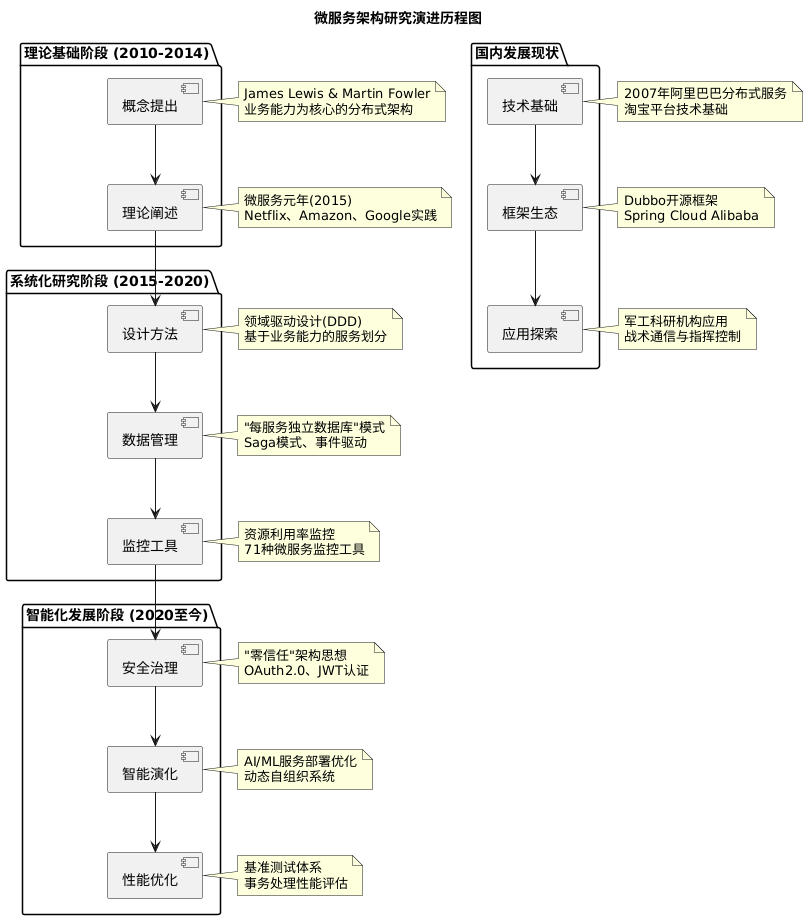
\includegraphics[width=0.9\textwidth,height=0.6\textheight,keepaspectratio]{chapters/fig-0/microservices_research_evolution.png}
    \caption{微服务架构研究演进历程图}
    \label{fig_microservices_research_evolution}
\end{figure}


\subsection{语义互操作}

语义互操作(Semantic Interoperability)作为异构系统间实现"语义层理解一致"的关键技术,其核心使命在于确保信息在跨系统、跨组织或跨领域传输过程中,不仅维持结构完整性,更能够被准确诠释与有效复用。这一概念的理论根基可追溯至语义网与本体论研究领域,通过构建形式化语义模型来刻画数据背后蕴含的概念体系及其关联关系,从而为复杂系统间的理解一致性奠定坚实的理论基础。伴随着信息系统复杂度的持续攀升与数据异构性的日益凸显,语义互操作已然演进为人工智能、云计算、医疗健康、工业物联网等诸多前沿领域的核心研究议题。

从国际研究视角审视,早期语义互操作研究主要聚焦于标准体系构建与模型分层设计。SISO、NATO 及 ISO 等权威机构率先提出的多层互操作模型,将信息交互过程系统性地划分为语法层、语义层与语用层三个层次\cite{SISO_STD_002_2006,CJCSI_6610_01F_2021},为后续研究奠定了统一的理论框架。步入 2010 年代,研究重心开始向本体(Ontology)在语义互操作中的核心作用转移。Mishra 与 Jain 创新性地提出了"语义知识宝库"(Semantic Knowledge Treasure)这一概念,通过运用 OWL 与 SPARQL 技术实现异构资源的统一语义表示与高效查询\cite{Mishra2018Semantic}。此类突破性研究的涌现,标志着语义互操作研究范式从概念层标准化向知识层深度融合的历史性转变。

进入近年来,知识图谱、人工智能与自动推理技术的蓬勃发展,推动语义互操作研究呈现出显著的智能化与自动化特征。Bernasconi 等人开创性地提出了"本体解包"(Ontological Unpacking)方法论,通过对现有概念模型进行深层次的本体剖析,有效揭示模型内部隐含的语义结构,从而显著提升模型的互操作性水平\cite{Bernasconi2022Ontological}。与此同时,Guizzardi 与 Guarino 在《Semantics, Ontology and Explanation》这一重要著作中深入探讨了语义互操作的解释性问题,强调应通过增强语义透明性与强化本体承诺(Ontological Commitment)来提升系统间的可理解性与信任度\cite{Guizzardi2023Explanation}。此外,将机器学习与规则引擎相结合的语义映射算法被广泛应用于自动发现概念对应关系,实现了跨领域知识的智能语义对齐与高效复用。

而随着云计算和分布式系统技术的广泛普及,语义互操作研究领域进一步向跨平台与多云环境扩展。Hamdan 与 Admodisastro 创新性地提出了一种基于本体的多云语义互操作参考架构,该架构通过引入语义中枢(Semantic Hub)这一核心组件来协调不同云平台的语义模型,从而实现服务间的语义一致性访问\cite{Hamdan2023Reference,Hamdan2024SemanticMultiCloud}。研究指出,在异构云环境中维持语义一致性需要在架构层、数据层与治理层之间建立有效的协同机制。更为重要的是,语义互操作正与数据治理、知识集成、可解释人工智能等前沿研究方向深度融合,为跨系统协同提供强有力的基础设施支撑。

从国内研究现状来看,语义互操作领域的研究工作起步于 2000 年代的语义网工程实践,近年来在知识图谱与人工智能技术快速发展的推动下呈现出加速发展的态势。研究内容主要涵盖语义本体构建、跨领域语义映射、语义检索与语义推理系统设计等关键方向。国内学者提出了基于知识图谱的语义关系建模框架,通过实体对齐与语义索引技术显著提升了异构数据的可融合性;同时,在智慧城市、医疗健康、交通运输和工业互联网等典型应用场景中,语义互操作技术被广泛应用于多源数据的协同管理与智能决策支持。当前研究趋势正从传统的"语义建模"向新兴的"语义计算"转变,更加关注语义理解、自动推理与动态本体演化的有机结合,以满足实时性、可解释性智能系统的迫切需求。

图\ref{fig_semantic_interop_research_trends}展示了语义互操作研究的发展趋势,全面梳理了从早期标准化阶段到智能化发展阶段的演进过程。该图详细展示了国外研究从2000-2010年的标准体系和模型分层,到2010-2020年的知识融合和智能映射,再到2020年至今的多云环境和语义中枢,以及国内从技术基础到应用场景再到发展趋势的研究路径,体现了语义互操作技术的理论深度和应用广度。

\begin{figure}[H]
    \centering
    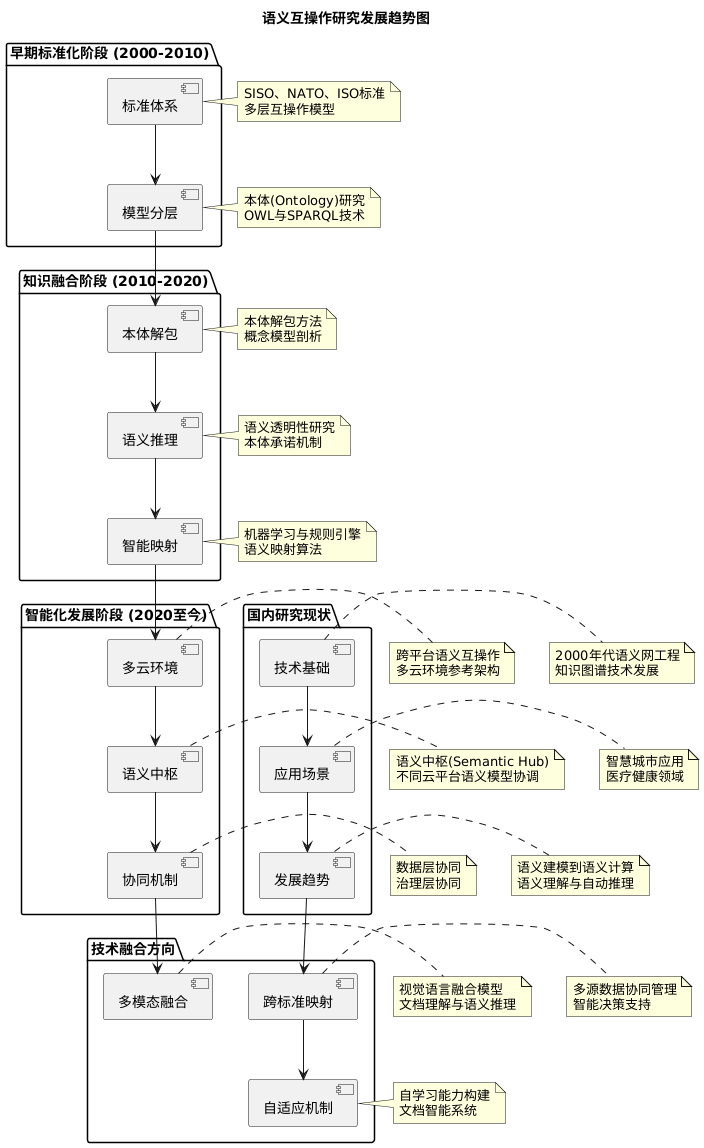
\includegraphics[width=0.9\textwidth,height=0.6\textheight,keepaspectratio]{chapters/fig-0/semantic_interop_research_trends.png}
    \caption{语义互操作研究发展趋势图}
    \label{fig_semantic_interop_research_trends}
\end{figure}


\subsection{文档自动化处理}

文档自动化处理技术作为复杂信息系统建设中的基础性支撑技术,其核心使命在于将非结构化或半结构化文档(如 PDF、Word、XML、JSON 等)进行智能解析、精准识别并高效导入数据库或知识系统,从而实现高效、准确的信息获取与结构化建模。这一技术领域的研究历程呈现出从传统基于规则的文档解析向现代机器学习与深度学习驱动的智能化处理的历史性转变,近年来在自然语言处理、文档智能(Document Intelligence)与多模态学习等前沿技术的强力推动下取得了突破性进展。

从技术发展脉络来看,早期自动化文档处理研究主要依托版面分析(Layout Analysis)和文本块识别等基础方法。代表性工作涵盖了基于光学字符识别(OCR)的文本抽取、表格检测与区域定位等核心算法。这一发展阶段的研究主要依赖于启发式规则与图像分割算法,如 PDFMiner、Apache Tika 等成熟工具框架,通过深入分析文本流与版面结构实现基本的内容解析功能。然而,这些传统方法在处理复杂文档中的语义结构与跨页逻辑关系方面仍存在显著局限性。

伴随着深度学习与自然语言处理技术的日趋成熟,研究重心开始向基于神经网络的文档理解与语义建模方向转移。自 2020 年以来,Google、Microsoft、Adobe 等国际知名机构相继推出了视觉语言融合模型(Vision-Language Models)用于文档解析。其中,Xu 等人提出的 LayoutLM 系列模型\cite{Xu2020LayoutLM,Huang2022LayoutLMv3},通过创新性地联合建模文本、位置与视觉信息,实现了对文档结构与语义的深层理解,在表格识别、关键信息抽取与文档分类等关键任务中得到了广泛应用。相关研究成果充分表明,基于 Transformer 架构的多模态模型在 PDF 结构分析中的性能表现显著优于传统方法,为复杂格式文档的自动化解析提供了通用性解决方案。

在信息抽取与结构化导入这一重要方向,学术界提出了多种智能抽取与标准映射框架。Rausch 等人在《DocParser: Hierarchical Document Structure Parsing from Renderings》这一重要文献中\cite{Rausch2021DocParser},创新性地提出了一种融合文本分块、实体识别与模板匹配的自动导入机制,成功实现了 PDF 与 XML 文档的语义级结构化导入。与此同时,研究者们将知识图谱构建技术与自动文档处理技术深度融合,通过实体识别、关系抽取与语义对齐等关键技术,实现了从原始文档到知识图谱的自动生成,为数据标准化与语义互操作奠定了坚实的技术基础。此类先进方法已在专利文档、医学报告与技术标准文件的自动建模过程中得到了有效验证。

进入近年来,自动化处理技术逐渐向自监督学习与跨模态理解这一前沿方向演进。现代模型系统不再过度依赖人工标注数据,而是通过大规模文档预训练实现通用特征学习能力。例如,Appalaraju 等人提出的 DocFormer 模型\cite{Appalaraju2021DocFormer},采用了文本与视觉双流 Transformer 的创新架构,在文档分类与表格提取等关键任务上达到了业界最优性能水平。更进一步的研究探索将大型语言模型(LLM)与文档理解技术深度融合,实现了跨模态语义推理与任务自适应能力\cite{Wang2023DocumentLLM},这一突破性进展标志着文档自动化处理正式进入"语义理解驱动"的全新发展阶段。

从国内研究现状审视,自动化文档处理领域的研究工作主要集中在结构化识别与智能导入系统的工程化实现方面。国内科研院所与企业界围绕 PDF 解析、表格抽取、字段标注与标准化导入等核心技术问题展开深入研究,成功开发了基于深度学习的 OCR 引擎与语义分层系统。例如,百度文心、阿里达摩院与华为诺亚方舟实验室等知名研究机构均提出了面向企业文档与技术标准的多模态解析解决方案,部分先进系统已在电子政务、科研档案与装备资料管理等重要领域中得到实际应用。尽管如此,当前国内研究仍面临跨格式迁移能力相对较弱、语义抽象层次有待提升、自动验证与错误纠正机制尚不完善等技术挑战,亟需在知识表示、语义约束与可解释性等关键方面进行深入探索。

综合而言,文档自动化处理技术正经历着从传统规则驱动向现代智能语义理解的历史性演进。国外研究在多模态模型、通用预训练与语义推理等前沿领域已形成相对完整的技术体系,而国内研究更多聚焦于工程应用与系统集成等实践层面。面向未来,技术发展趋势将重点聚焦于多模态语义融合、跨标准知识映射与自适应导入机制等关键方向,通过构建具备自学习能力的文档智能系统,最终实现技术标准、科研资料及战术数据等多源信息的自动解析与语义化导入。




\section{研究内容}

\subsection{研究的主要内容}

本文旨在设计和实现基于 MIL-STD-6016 的战术数据链信息标准数据库与语义互操作系统,通过对标准文档自动化处理、数据库架构设计、语义互操作机制和系统集成等方面的研究,实现一个高可靠、高性能、易扩展的战术数据链标准信息化平台,研究的主要内容如下:

(1)本文从系统的功能性需求分析入手,按照微服务架构的思想将系统分成若干个功能模块,并对各个功能模块使用需求分析工具用例图来详细描述需求。并且对系统的非功能性需求和部署需求进行了分析。针对 MIL-STD-6016 标准文档的复杂性和多样性,研究实现了基于适配器模式的六步流水线架构,支持多种标准的 PDF 文档自动解析\cite{MIL_STD_6016_Active_2024,MITRE_Link16_Interoperability_2024}。系统采用双路表格提取技术(Camelot + pdfplumber),结合智能章节识别与位段标准化算法,实现了从 PDF 文档到结构化 YAML 数据的全自动化转换。通过引入中间语义模型(SIM)与数据校验机制,确保处理结果的准确性与可追溯性。

(2)对本系统进行详细设计。根据系统的功能需求和业务特点,将系统划分为多个微服务,并选择合适的技术栈和框架进行开发。同时给出各个模块的具体业务流程,使用时序图和流程图等工具来详细描述设计结果。基于 MySQL 关系数据库构建了支持多标准消息存储与查询的信息标准数据库\cite{Laigner2021Data,Waseem2021Design}。数据库采用第三范式(3NF)设计,支持 J 系列消息、字段定义、编码规则及语义映射的统一管理。通过建立高效的索引策略与查询优化机制,系统能够支持大规模消息记录的结构化检索与跨字段模糊匹配,并实现多版本消息模型的差异比对与映射维护。

(3)根据系统设计的内容对系统功能进行实现。包括系统的各项功能模块的实现,并且实现日志收集分析模块、自动化部署模块等基础设施,以支撑系统的正常运行和高效管理。在语义互操作机制方面,研究实现了基于 Common Data Model(CDM)四层法的语义一致性框架,支持 MIL-STD-6016、MQTT、MAVLink 等不同协议间的消息转换\cite{Hamdan2023Reference,MITRE_Link16_Interoperability_2024}。系统通过概念层、协议层、消息层与字段层的分层映射,建立了可解释的跨标准语义绑定关系。同时,引入基于规则的智能路由与机器学习辅助的字段匹配算法,实现了高精度的语义对应识别与自动转换。

(4)对系统在功能和非功能两个方面进行测试,并对系统的性能进行评估。通过分析测试结果,用来验证系统的最终实现是否符合预期,为系统的上线和应用提供可靠的支撑。研究采用前后端分离的微服务架构,基于 FastAPI + React + TypeScript 技术栈构建了完整的 Web 应用系统\cite{Waseem2021Design,MonitoringTools2024}。后端提供 RESTful API 接口,支持 PDF 处理、消息转换、语义映射等核心功能;前端提供直观的可视化界面,包括 PDF 处理器、语义互操作接口、CDM 四层法界面等模块。系统支持与外部仿真平台、测试终端及网关设备的双向数据交互\cite{SAIC_JRE_Overview_2021,Collins_TTR_2021,L3Harris_STT_KOR24A_2020}。


\subsection{拟解决的关键问题}

基于对战术数据链标准信息化现状的深入分析,本研究致力于解决以下三个关键问题:

(1)标准数据的结构化与一致性问题:MIL-STD-6016及相关NATO标准文档包含大量嵌套的字段定义和复杂的比特位规则,传统的静态解析方法难以满足系统化建模的要求\cite{MIL_STD_6016_Active_2024,SISO_STD_002_2006}。针对这一问题,本研究提出自动化结构抽取与规范化建模方法,实现从标准文档到数据库的精确结构映射,确保数据的一致性和完整性。

(2)跨标准语义互操作问题:在多链并用和标准版本共存的复杂环境下,不同数据链协议间的语义差异成为制约系统互操作性的主要障碍\cite{Hamdan2023Reference,MITRE_Link16_Interoperability_2024}。为解决这一问题,研究引入基于CDM的统一语义层架构,通过规则推理与机器学习相结合的方法,实现字段级语义对应,确保数据在不同链路协议间保持语义一致性。

(3)系统性能与安全性保障问题:战术数据链数据库系统需要在高并发访问和实时响应条件下保持高可用性、安全性与稳定性\cite{Waseem2021Design,MonitoringTools2024}。针对这一挑战,研究采用分布式缓存、容器编排与加密通信等先进技术,构建高性能、高安全性的系统架构,确保系统在工程部署中的可靠运行。

基于上述关键问题,本研究设定了三个层次的目标。在理论层面,构建战术数据链信息标准数据库的统一建模与语义互操作理论框架,为跨链数据一致性提供方法论支持。在技术层面,设计高性能、可扩展的数据库与微服务系统,满足多标准融合与实时仿真验证的需求。在应用层面,通过数据库与仿真系统的联合应用,验证系统在态势共享与互操作性评估中的工程价值\cite{SAIC_JRE_Overview_2021,CurtissWright_TCG_HUNTR_2020,DOTE_2022_MIDS_LVT}。

\section{主要创新点}

本研究在战术数据链信息标准数据库系统设计与实现方面取得了以下四个方面的创新突破:

(1)自动化标准文档解析与结构化建模方法:面对MIL-STD-6016等复杂标准文档的解析挑战,本研究提出了基于深度学习的多模态文档理解方法。该方法融合OCR技术、表格识别算法和语义分析技术,成功实现了从PDF标准文档到结构化数据库的自动化转换。通过准确识别嵌套字段定义、比特位规则和约束条件,显著提升了标准数据录入的效率和准确性。

(2)基于CDM四层法的跨协议语义互操作框架:本研究将Common Data Model四层法引入战术数据链领域,构建了涵盖语义层、映射层、校验层和运行层的完整互操作架构。该框架通过建立统一语义概念库和智能映射规则,有效实现了MIL-STD-6016、MAVLink、MQTT等不同协议间的字段级语义对应,从根本上解决了传统方法中语义不一致的难题。

(3)微服务架构下的高性能数据存储与查询优化:本研究设计了基于微服务架构的分布式数据存储方案,采用MySQL主从复制、Redis缓存和Elasticsearch全文检索的混合存储架构。通过实施智能索引策略、查询优化算法和缓存预热机制,成功实现了毫秒级的数据查询响应,充分满足了战术数据链系统对实时性的严格要求。

(4)面向多标准融合的智能适配器设计:本研究提出了可插拔的协议适配器架构,该架构支持动态加载不同标准的数据处理模块。通过引入配置驱动的映射规则和机器学习辅助的字段匹配算法,实现了新标准的快速接入和现有标准的无缝升级,为系统的可扩展性和可维护性提供了强有力的技术保障。

\section{论文组织结构}

本文由六个章节组成,组织结构如下:

第1章为绪论,主要阐述基于MIL-STD-6016的战术数据链信息标准数据库系统的研究背景和意义。通过分析当前发展现状,识别出研究领域存在的关键问题。在此基础上,明确了本文的研究内容与目标,阐述了研究方法与技术路线,并概述了论文的整体组织结构。

第2章为相关工作,重点梳理战术数据链的发展历程和技术特点,深入分析MIL-STD-6016标准框架和J系列消息结构。此外,还系统介绍了微服务架构和语义互操作相关技术,为后续系统设计与实现奠定坚实的理论基础。

第3章为系统需求分析,从功能需求和非功能性需求两个层面展开分析。在功能需求方面,详细讨论战术数据链信息标准数据库系统所需的各种功能,并对这些功能进行深入分析和定义。在非功能性需求方面,从性能需求、安全需求、可扩展性需求等多个维度,为系统设计提供明确的目标和约束条件。

第4章为微服务架构与跨数据链协议互操作系统设计,基于前期需求分析结果,提出系统的总体架构设计方案。具体包括微服务架构设计与实现、数据模型与数据库设计,以及跨数据链协议互操作架构设计,从而构建完整的系统技术方案。

第5章为系统实现、测试与性能分析,详细阐述系统的实现过程,涵盖系统实现架构、后端服务实现、前端界面实现等关键技术环节。通过系统测试与实现验证,结合功能演示和性能测试,全面验证系统的有效性和实用性。

第6章为总结与展望,系统归纳基于MIL-STD-6016的战术数据链信息标准数据库系统设计与实现的研究成果,客观分析当前系统存在的不足之处,并对未来研究方向和改进措施进行展望,为后续系统升级提供参考。
